\documentclass[11pt]{labbook}
\usepackage[utf8]{inputenc}
\usepackage{graphicx}
\usepackage[margin=1.0in]{geometry}
\usepackage{setspace}
\usepackage{listings}
\usepackage{color}
\usepackage{array}
\usepackage{amsmath}
\usepackage{verbatim}
\usepackage[final]{pdfpages}
%%%%%%%%%%%%%%% Section for new commands %%%%%%%%%%%%%%%%%%%
\newcommand{\Loss}[2]{L\left(#1,#2\right)}

%%%%%%%%%%%%%%% End %%%%%%%%%%%%%%%%%%%%%%%%%%%%%%%%%%%%%%%%

\title{Lab Notebook}
\author{Alex Cope}
\date{August 2016}



\begin{document}
\maketitle
\let\cleardoublepage\clearpage
\tableofcontents
\labday{Mathematics and Statistics Notes}
 

\experiment{Chapter 7: Model Assessment and Selection}
Taken from \textit{The Elements of Statistical Learning}, 2nd ed, Hastie et al.
\subexperiment{7.2 Bias, Variance, and Model Complexity}
 
Let L(Y,$\hat{f}$(X)) be a loss function (can be squared error, absolute, etc), with X being a vector input, Y being a target vector, and $\hat{f}$(X) being estimated from some training set. Let $\mathcal{T}$ represent a training set. Then the test error is

\begin{align*}
Err_\mathcal{T} &= E\left[L\left(Y,\hat{f}(X)\right)|\mathcal{T}\right]
\end{align*}

which is the prediction error over an independent sample. Note that X and Y are drawn from their joint distribution. The expected test error is 

\begin{align*}
Err &= E\left[L\left(Y,\hat{f}(X)\right)\right] = E\left[Err_\mathcal{T}\right]
\end{align*}

Err is better for statistical analysis and most methods estimate this quantity. 
\newline

Training error:

\begin{align*}
\overline{err} &= \frac{1}{N}\sum_{i=1}^{N}\Loss{y_i}{\hat{f}(x_i)}
\end{align*}


As model complexity increases, training data is used more and adapts to more complicated information extracted from the model; however, this drives down the bias but increases the variance. Want to minimize expected test error. 

Training error is not a good estimate of test error. In fact, a model with a training error of 0 is an overfit, meaning it will perform poorly when working with other data sets. 

What if we are working with categorical data. The situation is very much the same. Let $\Loss{G}{\hat{G}(X)}$ (G = $\hat{G}$(X) = $argmax_k$ $\hat{p}_k$(X)) be a loss function, where G is a categorical response taking one of K values. Let $p_k(x)$ be the probability that G = k given the input X. A loss function in this case might be 0-1 loss or something more complex (see pg. 221).

Training error for this type of data is 

\begin{align*}
\overline{err} = -\frac{2}{N}\sum_{i=1}^{N}log\hat{p}_{g_i}(x_i)
\end{align*}

The log-likelihood can serve as a loss-function for Poisson, gamma, exponential, and log-normal. From my understanding, this is essentially what ROC and similar models do when sampling gene expression values. Let $Pr_{\theta\left(X\right)}$(Y) be the density of Y, indexed by $\theta$(X), then

\begin{align*}
\Loss{Y}{\theta(X)} &= -2 \cdot logPr_{\theta\left(X\right)}(Y)
\end{align*}

\subexperiment{7.3 The Bias-Variance Decomposition} 
Let Y = f(X) + $\epsilon$, where the average value of $\epsilon$ is 0 and the variance is equal to $\sigma_\epsilon^2$. Then with a regression $\hat{f}$(X) at point $x_0$ with squared error loss, the expected prediction error is 

\begin{align*}
Err(x_0) &= Irreducible Error + Bias^2 + Variance
\end{align*}

where the first term is the variance of the target around true mean f($x_0$), the second is the amount by which the estimate differs from the true mean, and the third is the expected squared deviation of $\hat{f}(x_0)$ around its mean. Generally, the more complex $\hat{f}$, the lower the squared bias but the higher the variance. 

The biggest thing to take from this section is that as model complexity goes up, squared bias generally decreases, but variance increases. 


\subexperiment{7.4 Optimism of the Training Error Rate}
Typically, the training error is less than the true error because same data used to fit and assess the model. 

Define the \textit{in-sample error} to be
\begin{align*}
Err_{in} &= \frac{1}{N}\sum_{i=1}^{N}E_{Y^0}\left[\Loss{Y_i^0}{\hat{f}(x_i)}|\mathcal{T}\right]
\end{align*}

$Y^0$ indicates N new responses for N training points. Let the \textit{optimism} and its corresponding average over training sets \textbf{y}, $\omega$, be
\begin{align*}
op \equiv Err_{in} -\overline{err} \\
\omega \equiv E_{\textbf{y}}(op)
\end{align*}
which is usually a positive term since the training error is usually driven down by fitting/assessment approach. Usually can only estimate $\omega$. For many common loss functions (including squared error),

\begin{align*}
\omega &= \frac{2}{N}\sum_{i=1}^{N}Cov\left(\hat{y}_i,y_i\right)
\end{align*}
In summary, the expected value of the in-sample error is the sum of expected value of the training error over training sets \textbf{y} and $\omega$,
\begin{align*}
 E_{\textbf{y}}(Err_{in}) &= E_{\textbf{y}}(\overline{err}) + \frac{2}{N}\sum_{i=1}^{N}Cov\left(\hat{y}_i,y_i\right)
\end{align*}   

If $\hat{y}_i$ is obtained via linear fit with d inputs, then,
\begin{align*}
\sum_{i=1}^{N}Cov\left(\hat{y}_i,y_i\right) &= d\sigma_{\epsilon}^{2} \\
\rightarrow  E_{\textbf{y}}(Err_{in}) &= E_{\textbf{y}}(\overline{err}) + 2 \cdot \frac{d}{N}\sigma_{\epsilon}^{2}
\end{align*}
Optimism increases linearly with number of inputs, but decreases as training set increases in size. 

\subexperiment{7.5 Estimates of In-Sample Prediction Error}
Let d parameters be fit under squared error loss, then you get the $C_p$ statistic,
\begin{align*}
C_p &= \overline{err} + 2 \cdot \frac{d}{N}\hat{\sigma}_{\epsilon}^{2}
\end{align*}

Note: $\hat{\sigma}_{\epsilon}^{2}$ is estimate of the noise variance.
\newline
\newline
\textbf{Akaike information criterion (AIC)}:\newline

Used to estimate $Err_{in}$ when using log-likelihood loss function. 

\begin{align*}
-2 \cdot E\left[logPr_{\hat{\theta}}(Y)\right] &\approx -\frac{2}{N} \cdot E\left[loglik\right] + 2 \cdot \frac{d}{N} \\
\hat{\theta} &= MLE(\theta) \\
loglik &= \sum_{i=1}^{N}logPr_{\hat{\theta}}(Y)
\end{align*}

where $Pr_{\theta}$(Y) is a family of densities for Y (one of which is the true density).

When selecting a model via AIC, choose one that minimizes AIC. It is important to note that when using nonlinear models, d must be replaced with some measurement of model complexity. 

In general, let $\mathcal{F}$ be a set of models $f_{\alpha}$(x), where $\alpha$ is a tuning parameter. Then,
\begin{align*}
AIC(\alpha) &= \overline{err}(\alpha) + 2 \cdot \frac{d(\alpha)}{N}\hat{\sigma}_{\epsilon}^2
\end{align*}
Basically, AIC estimates the test error curve, so you want to find the $\hat{\alpha}$ that minimizes it. 

Book notes that if basis functions are chosen adaptively, this whole thing collapses. 
\newline

Example) You have p total inputs, but best fitting linear model takes $d<p$ inputs, optimism will exceed (2d/N)$\sigma_{\epsilon}^{2}$.

\subexperiment{7.7 The Bayesian Approach and BIC}
Like AIC, applicable where fitting occurs via maximizing log-likelihood (ie. what we are doing with ROC). Generic form of BIC:

\begin{align*}
BIC &= -2 \cdot loglik + \left(log N\right) \cdot d
\end{align*}

Under a Gaussian model ($\sigma_{\epsilon}^2$ is known), $-2 \cdot loglik$ equals up to a constant $\sum_i^N(y_i -\hat{f}(x_i))/\sigma_{\epsilon}^2$. For a squared error loss, this is $N \cdot \overline{err}/\sigma_{\epsilon}^2$
\begin{align*}
\rightarrow BIC &= \frac{N}{\sigma_{\epsilon}^2}\left[\overline{err} + \left(log N\right) \cdot \frac{d}{N}\sigma_{\epsilon}^2\right] \\
\rightarrow BIC &\propto AIC
\end{align*}

BIC tends to penalize complex models, but as $N \rightarrow \infty$, the probability BIC picks correct model goes to 1.



\experiment{Chapter 6: Model Checking}
\subexperiment{6.1 The place of model checking in applied Bayesian statistics}

\textit{Sensitivity Analysis} - how much do posterior inferences change in our model versus other models

\subexperiment{6.2 Do the inferences from the model make sense?}

\underline{Checking model via external validation} \newline
$\bullet$	Use model to make predictions, collect actual data, do they match up? \newline
$\bullet$ Usually need to check model \textbf{before} getting new data

\subexperiment{6.3 Posterior predictive checking}

To measure discrepancy between models and data, define test quantity T(y,$\theta$). Think test statistic in frequentist hypothesis testing, which depends only on data. To measure lack of fit of data with respect to posterior predictive distribution can be measured as p-value of test quantity. In a Bayesian framework, the p-value is 

\begin{align*}
p_B &= Pr(T(y^{rep},\theta) \geq T(y,\theta)|y)\\
&= \iint{I_{T(y^{rep},\theta) \geq T(y,\theta)}p(y^{rep}|\theta)p(\theta|y)dy^{rep}d\theta}
\end{align*}

which translates to the probability a set of replicated data could be more extreme than the observed (\textbf{how is this different from the frequentist's definition?}). A p-value can be calculated via simulations: drawing from joint posterior distribution, the p-value is simply the ration of

\begin{align*}
T(y^{rep s},\theta) \geq T(y,\theta^s)
\end{align*}

where the $y^{rep s}$ are drawn from the simulated values of $\theta^s$.

\experiment{Chapter 7: Evaluating, comparing, and expanding models}

\subexperiment{7.1 Measures of predictive accuracy}
Measures of predictive accuracy should be guided by the application:
$\bullet$ point prediction - single value reported as prediction of future observation (mean squared error)
\newline
$\bullet$ probabilistic prediction - report inferences about $\tilde{y}$ that takes into account full uncertainty over $\tilde{y}$
\newline

Log-likelihood, $\log{p(y|\theta)}$, is a probabilistic prediction. Proportional to the mean squared error if model is normal with constant variance. With large sample sizes, minimizing Kullback-Leibler information is the same as maximizing expected log-likelihood. Use log-likelihood because of its generality and because we are interested in summarizing the model fit to data (prior density is not relevant in computing predictive accuracy). 
\newline
\newline
\underline{Ideal measure of model fit: predictive performance for new data (external validation).} 
\newline

Let:\newline
$\bullet$ f be the true model \newline
$\bullet$ y be the observed data \newline
$\bullet$ $\tilde{y}$ be the future/alternative data

Out-of-sample predictive fit for new data point $\tilde{y}_i$ is
\begin{align*}
\log{p_{post}(\tilde{y}_i)} &= \log{E_{post}(p(\tilde{y}_i|\theta))}\\
&= \log{\int p(\tilde{y}_i|\theta)p_{post}(\theta)d\theta}
\end{align*}
where $p_{post}(\tilde{y}_i$ is the predictive density and $p_{post}(\theta)$ is the posterior. 

Expected out-of-sample log-likelihood, since future data unknown:
\begin{align*}
E_f(\log{p_{post}(\tilde{y}_i)}) &= \int(\log{p_{post}(\tilde{y}_i)})f(\tilde{y}_i)d\tilde{y}
\end{align*}

Generally, $\theta$ is not known, so can't get $\log{p(y|\theta)}$. Want to summarize predictive accuracy with
\begin{align*}
\log{\prod p_{post}(y_i)} &= \sum_{i=1}^n \log{\int p(y_i|\theta)p_{post}(\theta)d\theta}
\end{align*} 
which is usually computed in practice by generating $\theta^s, s = 1,...,S$ from $p_{post}(\theta)$ and then
\begin{align*}
\sum_{i=1}^n \log{\left(\frac{1}{S} \sum_{s=1}^S p(y_i|\theta^s)\right)}
\end{align*}

\subexperiment{7.2 Information criteria and cross-validation}

\textit{Information criteria} typically defined based on deviance = $-2\log{p(y|\hat{\theta})}$ 

Interested in prediction accuracy for model validation and comparing models. \textbf{From pg. 170 of BDA: "When different models have the same number of parameters estimated in the same way, one might simply compare their best-fit log predictive densities directly,"...So in my current case, can I just compare the log-likelihoods of the different ROC results?}

Can approximate out-of-sample predictive accuracy using existing data:

1) \textit{Within-sample predictive accuracy} - Naive estimate of log-likelihood for new data is log-likelihood of existing data. In general, overestimate

2) \textit{Adjusted within-sample predictive accuracy} - Corrections for bias in computed log-likelihood based on existing data and is approximately unbiased. Corrects bias by subtracting off biases produced via number of (effective) parameters being fit. Reasonable, but correct at best only in expectation

3) Cross-validation


Gelman et al recommend using WAIC as a measure of predictive performance, which is a more Bayesian approach than AIC or DIC. WAIC has the property that it averages over the posterior distribution, as opposed to conditioning on a point estimate. 

\begin{align*}
p_{WAIC} &= 2 \sum_{i=1}^n\left(\log{(E_{post}p(y_i|\theta))} - E_{post}(\log{p(y_i|\theta)})\right) \\
computed\ p_{WAIC} &= 2 \sum_{i=1}^n\left(\log{\left(\frac{1}{S} \sum_{s=1}^S p(y_i|\theta^s)\right)} - \frac{1}{S}\sum_{s=1}^S\log{p(y_i|\theta^s)}\right)
\end{align*}

They also DO NOT recommend using BIC, as the goal of this criterion is to approximate the marginal probability density of the data p(y) under the model, which can then be used to estimate relative posterior probabilities. 

\labday{Computer Science Notes}

\experiment{Working with Pandas (Python package)}


\labday{Biology Notes}

\experiment{Journal club: \textit{Integrative proteomic profiling of ovarian cancer
cell lines reveals precursor cell associated proteins
and functional status}}

Difficult to perform mechanistic studies with primary tissue, so need cellular models. Models need to be representative of tumor. 

Genomic/Transriptomic analyses do not necessarily reflect proteomic profile. 

Use streamline MS-based proteomics approach for molecular subtype characterization.

Many OvCa cell lines have been assigned to the wrong tissue of origin. 


~229,000 unique peptide sequences $\rightarrow$ 11,070 distinct protein groups (FDR < 1%). 

Look into Label-free protein quantification. 

Used clustering based on expression of ~8,500 distinct proteins quantified in at least 10 of 30 cell lines, which resulted in three main groups:\newline
 1) Group 1: cells lines previously reported to represent HGSOC cell lines based on genomic profiles\newline
 2) Group 2: unlikely HGSOC lines \newline
 3) Group 3: Note how some of the cell lines in this group are related, but doesn't address how all of them are related, so why is this not split up into multiple groups
 
Expected two cell lines to cluster in group 1 based on genomic similarity to HGSOC tumors, but instead were in group 3. They hypothesize that there is a discriminating feature of these tumors only visible at protein level.

Used principal component analysis at whole-proteome levels, which also showed three groupings. Determined 67 proteins with highest discriminating power between groups using feature selection and SVMs. 

\subexperiment{Sarvesh's presentation}
Incorrect tissue origin:
$\bullet$ cell lines representative of tumor \newline
$\bullet$ 30 years since ovarian cell lines have been established \newline
$\bullet$ cross-contamination 

Goal of study: Integrated/streamlined MS-based proteomics approach for linking proteomic profiles from cell lines, tumor tissues and primary cells for evaluation of OvCa cellular model systems.

Functional signature are at protein and metabolite level.

Longer chromatography dilutes sample more, For narrow peak, MS might scan twice and then able to get new peak. Broader peak will be scanned by MS more, becomes redundant. 


\labday{Progress Tracker}
\experiment{8-25-2016}
\subexperiment{Reading}
1. Li \textit{et al}.
Whole genome analysis of non-optimal codon usage in secretory signal sequences of \textit{Streptoyces coelicolor}. \textit{Biosystems}. 2006
\newline
2. Zalucki \textit{et al}. Secretory signal sequence non-optimal codons are required for expression and export of b-lactamase. \textit{Biochemical and Biophysical Research Communications}. 2007
\newline
3. Read Chapter 2 out of Lynch 2007.
\let\cleardoublepage\clearpage

At Cedric's recommendation, I re-ran the \textit{E. coli} simulations with more samples (10,000 up to 50,000). He pointed out that the frequency plots for the codon usage were a little flat, which would be reflected in the traces not converging. The traces looked okay, but I decided it wouldn't hurt to rerun them with a few more samples. The plots looked almost identical, so it seems like 10,000 samples is sufficient for the \textit{E. coli} genome. One of the peptides that looks particularly flat is for Lysine (K). The AAA codons is favored at a frequency of ~0.8, regardless of log$\phi$. In \textit{E. coli}, AAA is the best initiator of translation. I wonder if this plays a role in the strong bias for AAA.
\newline
Also ran for \textit{C. bescii} and received the data on \textit{E. coli} gene expression from the Li 2014 paper.
\newline
Mallory Ladd (in Bob's lab) asked me to write some scripts from her for a project she is working on last week. She reminded me on today, so I decided to finish that up. Most of the scripts were based on work I did during my rotation in Bob's lab, but her files were in a different format. This required me to make modifications to my previous scripts, which turned out to be more annoying than I thought it would be.

\experiment{8-26-2016}
Finished up the scripts for Mallory and ran them for her. When I have a chance during the weekend, I will spend time learning how to use LaTeX, grading the short essays I assigned my students on the role of computation in unlocking biological systems, and finish preparing for lab on Monday.
\newline

Also, touched base with Steve regarding the protein clustering project he and I worked on during my rotation. He is collaborating on a similar project with Dr. Barerra over in BCMB and said he is planning on giving the project to an undergrad. After the undergrad has done some initial calculations, he said I'm welcome to help out on creating some "relatively low hanging" simulation code. Depending on how work is progressing with my other projects, I would like to help out on this where I can. 

\subexperiment{Goals for next week}
1. Compare gene expression results from ROC simulations with results from Li 2014.
\newline
2. Look at gene expression results for the genes with predicted signal peptides. See if the majority of them are low expression genes (ie. non-optimal codon usage could be largely due to mutation biases).
\newline
3. Begin thinking about how to handle house-keeping genes in current models.
\newline
4. Resume independent-study of Bayesian Data Analysis.


\experiment{8-29-2016}
Next steps for analysis:\newline
1) Fit model to genome consisting of genes with the first 35 amino acids removed, which should eliminate most of the signal peptide components. I would expect that if signal peptides have evolved under different selective pressures, then the overall model fitting would improve. However, given the large size of most genes relative to the signal peptides, I don't know how much impact removing these will have even if the signal peptide region and the rest of the gene are evolving differently. 

2) Fit model to just genes with predicted signal peptides and do a separate model fitting to genes without predicted signal peptides. If genes with signal peptides are evolving differently, I would expect to see a drop off in the fitting relative to the genes without signal peptides. The number of genes with predicted signal peptides is roughly 10 percent of the E. coli genome (425 genes), so I don't know if this will be enough to get accurate fittings. Maybe I could create a random subset of 425 genes without signal peptides and fit the model to this subset in order to eliminate size as a variable in the analysis.

3) I would like to perform analysis with the mixture models that we discussed yesterday. It makes sense to me to treat genes with signal peptides vs those without as separate subpopulations within the genomes. I'm also wondering if it would be possible to go a level deeper in this analysis and treat individual codons as a member of a signal peptide vs a non-signal peptide. To me, this seems like a more accurate approach since it is the regions within the gene that could be evolving differently. However, my understanding of mixture models is limited and my knowledge of the current implementation in ROC even less so. Currently reading Gelman's chapter on Finite Mixture Models in order to improve my understanding. 

\experiment{8-30-2016}
Submitted the above to Mike here are his responses.

1) Only one way to find out.  Key question is how will you compare the quality of the model fits? 

Me: Read up on model checking in Gelman's book

2) Creating a 'control' set makes sense, but note that the quality of the fit is quantitatively described by the  posterior parameter intervals (more info, tighter intervals) and measures of model fit based on the unscaled probabilities of the MCMC samples.

3) For the first part, I would agree this would be a good step. If you use the mixture model approach, you can initially designate genes into particular category and let the algorithm update these designations.  Preliminary work 
suggests that using estimates of $\phi$'s when fitting the model helps with the categorization.

Me: Have this from Li et al (2014, Cell). 

For the second part, I agree that trying to apply separate models to different parts of the gene would be nice.  How to do this in the current framework will take some thought.  Note that I am interested in a similar type of analysis at the level of separate introns for alternatively spliced 
genes. 

Completed a run of the truncated genome, but a problem occurred when trying to plot these functions. Mike suggested I look into writing the objects to a file. Looked into the parameterObject.r class and found a writeParameterObject function, which seems to accomplish this task. Added it to my standard template script for running ROC. Now if something happens when plotting or I want to go back to do more analysis on a run, this object will be saved to a file. 

Mike noted that I need to understand where the sources of the data come from. Li et al (2014, Cell) performs their subexperiments using ribosome footprinting. The mRNA levels they provide are RPKM values, which are normalized by the length of the gene. 


\experiment{8-31-2016}
Towards the end of the day, got the following error while attempting to fit ROC to a genome consisting of only genes containing signal peptides. When the the function to plot the CUB plot was called, I got a memory allocation issue with the following traceback:

*** caught segfault ***
address 0xfffffffffffffff8, cause 'memory not mapped'
\newline
Traceback:\newline
1: .External(list(name = "CppMethod\_\_invoke\_notvoid", address = <pointer: 0x2cdce60>,     dll = list(name = "Rcpp", path = "/usr/lib/R/site-library/Rcpp/libs/Rcpp.so",         dynamicLookup = TRUE, handle = <pointer: 0x2df0a00>,         info = <pointer: 0x7f3a5ebf9860>), numParameters = -1L),     <pointer: 0x238f690>, <pointer: 0x23a9af0>, .pointer, ...)
\newline
2: genome\$getGenomeForGeneIndices(genes.in.mixture, simulated)
\newline
3: plot.Rcpp\_ROCModel(model, genome, samples = samples * 0.1, mixture = 1,     main = "E.coli Codon Usage Plot")\newline
4: plot(model, genome, samples = samples * 0.1, mixture = 1, main = "E.coli Codon Usage Plot")
 \newline
 
I ran this on Gauley with the most up-to-date version of the RibModel. I moved this file over to my computer with a slightly old version and did not get this error. I sent Holis all the information I could in hopes that he could figure out what is going on.

\experiment{9-1-2016}
Based on my conversations with Mike, it seemed like if I wanted to continue a fitting, I could load Parameter and MCMC objects from previous runs. I have no problem doing this with just a MCMC object, but if I try to continue a fitting using a loaded Parameter object, I get another memory allocation issue with the following traceback:
\newline
 *** caught segfault ***
address (nil), cause 'memory not mapped'
\newline
Traceback:\newline
 1: .External(list(name = "CppMethod\_\_invoke\_void", address = <pointer: 0x2715d50>,     dll = list(name = "Rcpp", path = "/usr/local/lib/R/site-library/Rcpp/libs/Rcpp.so",         dynamicLookup = TRUE, handle = <pointer: 0x28a8f20>,         info = <pointer: 0x7f02b49b4b40>), numParameters = -1L),     <pointer: 0x406d990>, <pointer: 0x32e5060>, .pointer, ...)
\newline 
 2: mcmc\$run(genome, model, ncores, divergence.iteration)
\newline
 3: runMCMC.Rcpp\_MCMCAlgorithm(mcmc, genome, model, 4)
\newline
 4: runMCMC(mcmc, genome, model, 4)
\newline
 5: system.time(runMCMC(mcmc, genome, model, 4))
\newline
 6: eval(expr, envir, enclos)
\newline
 7: eval(ei, envir)
\newline
 8: withVisible(eval(ei, envir))
\newline

Since I've been wanting to get into the code a little more, I figured trying to debug this myself wouldn't be a bad idea. Based on what I found, it seems like the writeParameterObject() function in R is intended to create a Parameter object that will be used \textbf{just} for future data analysis, not a starting point for a new run. Maybe that is what was intended, but I think this is bad software practice. If you have two objects of the same class, then they should work the same way.

The place where things are breaking is at the call for ROCModel::updateTracesWithInitialValues(Genome \&genome). The source of this error seems to be that many of the variables that are needed for fitting a model are initialized in the initParameterSet() function. This function is only called from the constructors of the Parameter subclasses; as a result, they will only be initialized when the initializeParameterObject() is called in R. 

The loaded Parameter object does not see groupList, which is an array containing the amino acid letter ids (ie. K for lysine). This can be fixed by moving the initialization of this list to the Parameter.h file. I still need to do some digging into this.

\experiment{9-2-2016}
I continued some of the debugging from yesterday. I also was unfortunate enough to encounter the error from August 31st again on my local machine. However, I have not had much luck consistently generating this error, so what the cause of it is baffling me. 

However, I did find a fairly significant error in  Genome::getGenomeForGeneIndicesR(), which returns a genome consisting of the genes in a mixture. In the plotModelObject.R (generates CUB plots), it looks like it pulls out the genes in a mixture and passes into Genome::getGenomeForGeneIndicesR() a list of the indices for these genes. The problem is these indices are based on an R vector (starts at 1), but the code in Genome::getGenomeForGeneIndicesR() forgets to subtract off 1 to convert the indices to C++ array indices (starting at 0). In the case of a mixture model with only 1 category, this just means the genome returned will be missing the fist gene and contain a blank gene in the last position in the gene array. However, when fitting using mixture categories, this means you could be missing a lot of genes. I'm not surprised this error was not found sooner because of C/C++ not returning an IndexOutOfBounds error when accessing array/vector elements via array[index]. It is generally safer when working with std::vector<> to use vector.at(index), as this will return an IndexOutOfBounds error. However, it is also slower. 

I talked with Bob before I called it a day. I explained to him some of the problems with previous analysis of codon usage bias for signal peptides in \textit{E. coli} (ie. failure to account for affects of varying gene expression) and showed him some of the plots I generated. I also explained to him the next steps I want to take with the analysis. He said he was happy about what I have done so far and where I plan on going with this project.

\subexperiment{Plans for Weekend}
Continue reading "Part 2: Fundamentals of Bayesian Data Analysis" from \textit{Bayesian Data Analysis}, 3rd ed, Gelman et al and "Chapter 7: Model Assessment and Selection" from \textit{The Elements of Statistical Learning: Data Mining, Inference, and Prediction}, 2nd ed, Hastie et al.

Also review the chapter on numerical integration from \textit{Numerical Methods}, 4th ed, Faires and Burden. This thing about dividing a Gamma distribution up into quantiles and taking the average value of each just seems wrong to me. 

\experiment{9-6-2016}
Focused on learning about model checking. I just want to get a solid base in this area by the end of this week so I can start implementing some model checks. So far, looking like the Bayesian Information Criterion (BIC) might be a good start, but I want to read up on it a little bit more. I know Gelman et al talks about it and Hastie et al cite the original paper, which also might be worth taking a look at. 

Last week, Mike noted that sometimes it is hard to tell if the traces are actually converging based on the plots. I think adding a moving average function might make this task a little bit easier. 

In one of the earlier SignalP paper, the authors note that SignalP should not be used to identify extracellular proteins; instead, researchers should use SecretomeP (by the same group). This brings up a good point: most of the papers that have done analysis of codon usage bias in signal peptides have seemed to imply that signal peptide = extracellular. It might be worth dividing up those with signal peptides into two groups: those that are predicted to be extracellular via SecretomeP and those that are not and fit these in ROC with a mixture model. 

\experiment{9-7-2016}
Talk to Cedric about autocorrelation functions. Look at Geweke scores. 


\experiment{9-11-2016}
Since 9-7-2016:
$\bullet$ Set up a Github repository for Bob's lab. Should make it easier for us to keep track of the scripts we write and make accessing them easier. I also commented/documented some of the scripts I had previously written to make them more accessible to my labmates who have little programming experience. \newline
$\bullet$ Got a little bit of experience working with the Python package, Pandas. Supposed to be good for data analysis, which is why Yaojin has suggested teaching it in LFSC 507. \newline
$\bullet$ Looked into autocorrelation functions and MCMC checking methods, including the Geweke score. \newline
$\bullet$ Performed an autocorrelation on the $\Delta\eta$ and $\delta$M traces using R's acf function. Generally, they looked something like this.

\includepdf[pages=8]{Autocorrelation_just_genes_w_sigpep.pdf}

$\bullet$ I also ran the acf for the loglikelihood trace and also got good results.

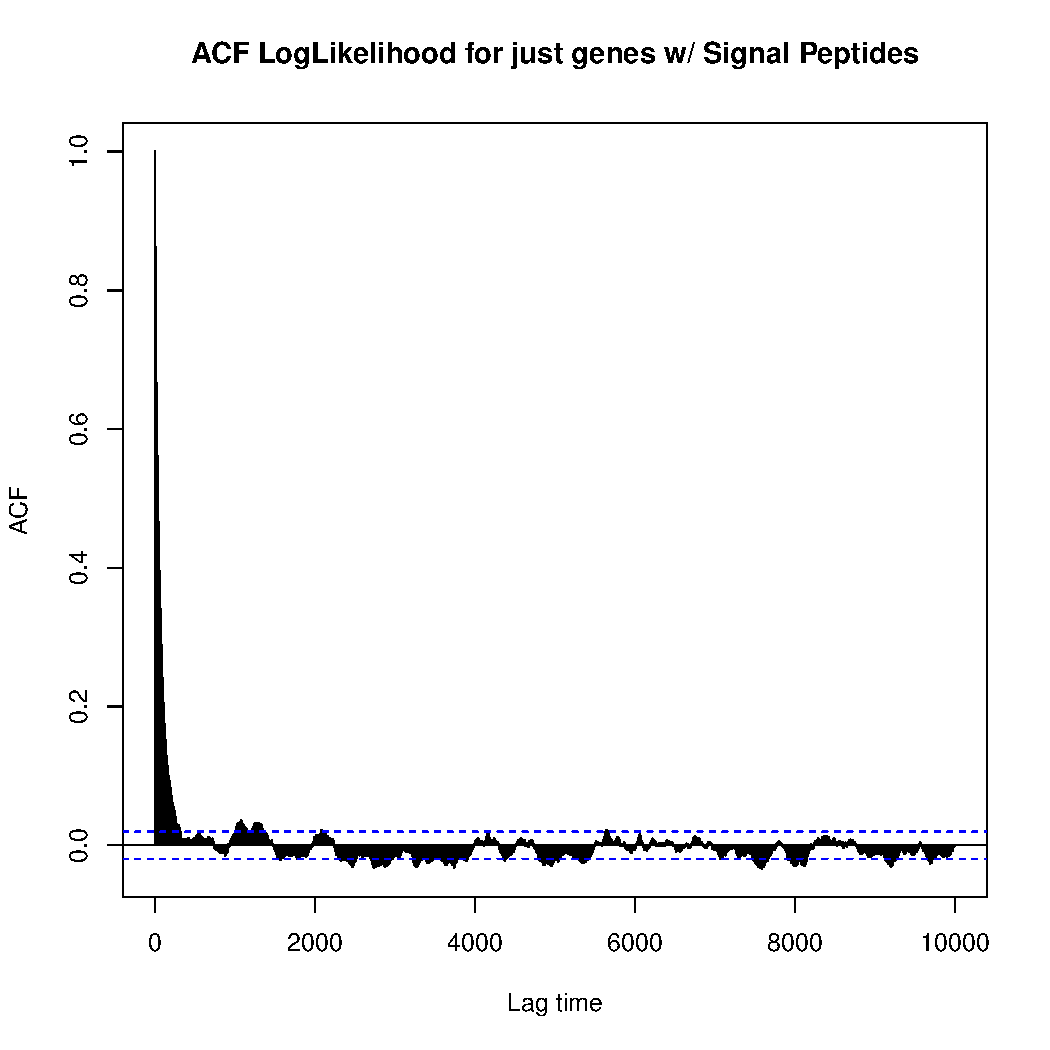
\includepdf[pages=1]{acf_loglikelihood.pdf}


\end{document}